\section{Application 2} \label{sec:case_study2}

In this section, results analysis related to the four experiments is presented. The first experiment (Section~\ref{subsec:propVSprop}) is conducted to compare the performance of the proposed approach when employing different preprocessing techniques. The second (Section~\ref{subsec:propVSdecomp}) compares the performance of the proposed model with those that only use \ac{CEEMD}. The third experiment (Section~\ref{subsec:propVSstack}) aims to compare the performance of the proposed model with the \ac{STACK} models. The last investigation (Section~\ref{subsec:propVSmodels}) compares the proposed model's performance against non-decomposed models. By running all these comparisons, the forecasting accuracy of the proposed framework can be effectively evaluated. In Tables \ref{tab:PROPversusCEEMD}, \ref{tab:PROPversusSTACK}, and \ref{tab:PROPversusMODELS}, on Appendix~\ref{app:hyper}, the best results are highlighted in bold. Further, Tables~\ref{tab:hyper1_cs2} and \ref{tab:hyper2_cs2}, also on Appendix~\ref{app:hyper}, present the hyperparameters of the models used in this study. A grid-search defined the best tunes of the hyperparameters for the base and meta-learner.

\subsection{Comparison with different preprocessing techniques \label{subsec:propVSprop}}

The first comparison evaluates the performance of the forecasting models that employed the proposed learning framework, the models that employed the decomposition, and the stacking-ensemble learning techniques. The models were performed using different preprocessing techniques. The proposed models are named \ac{CEEMD}--\ac{BC}--\ac{STACK}, \ac{CEEMD}--\ac{CORR}--\ac{STACK}, and \ac{CEEMD}--\ac{PCA}--\ac{STACK}, respectively.

% Figures MAPE of CEEMD-STACK
\begin{figure}[htb!]
    \centering
    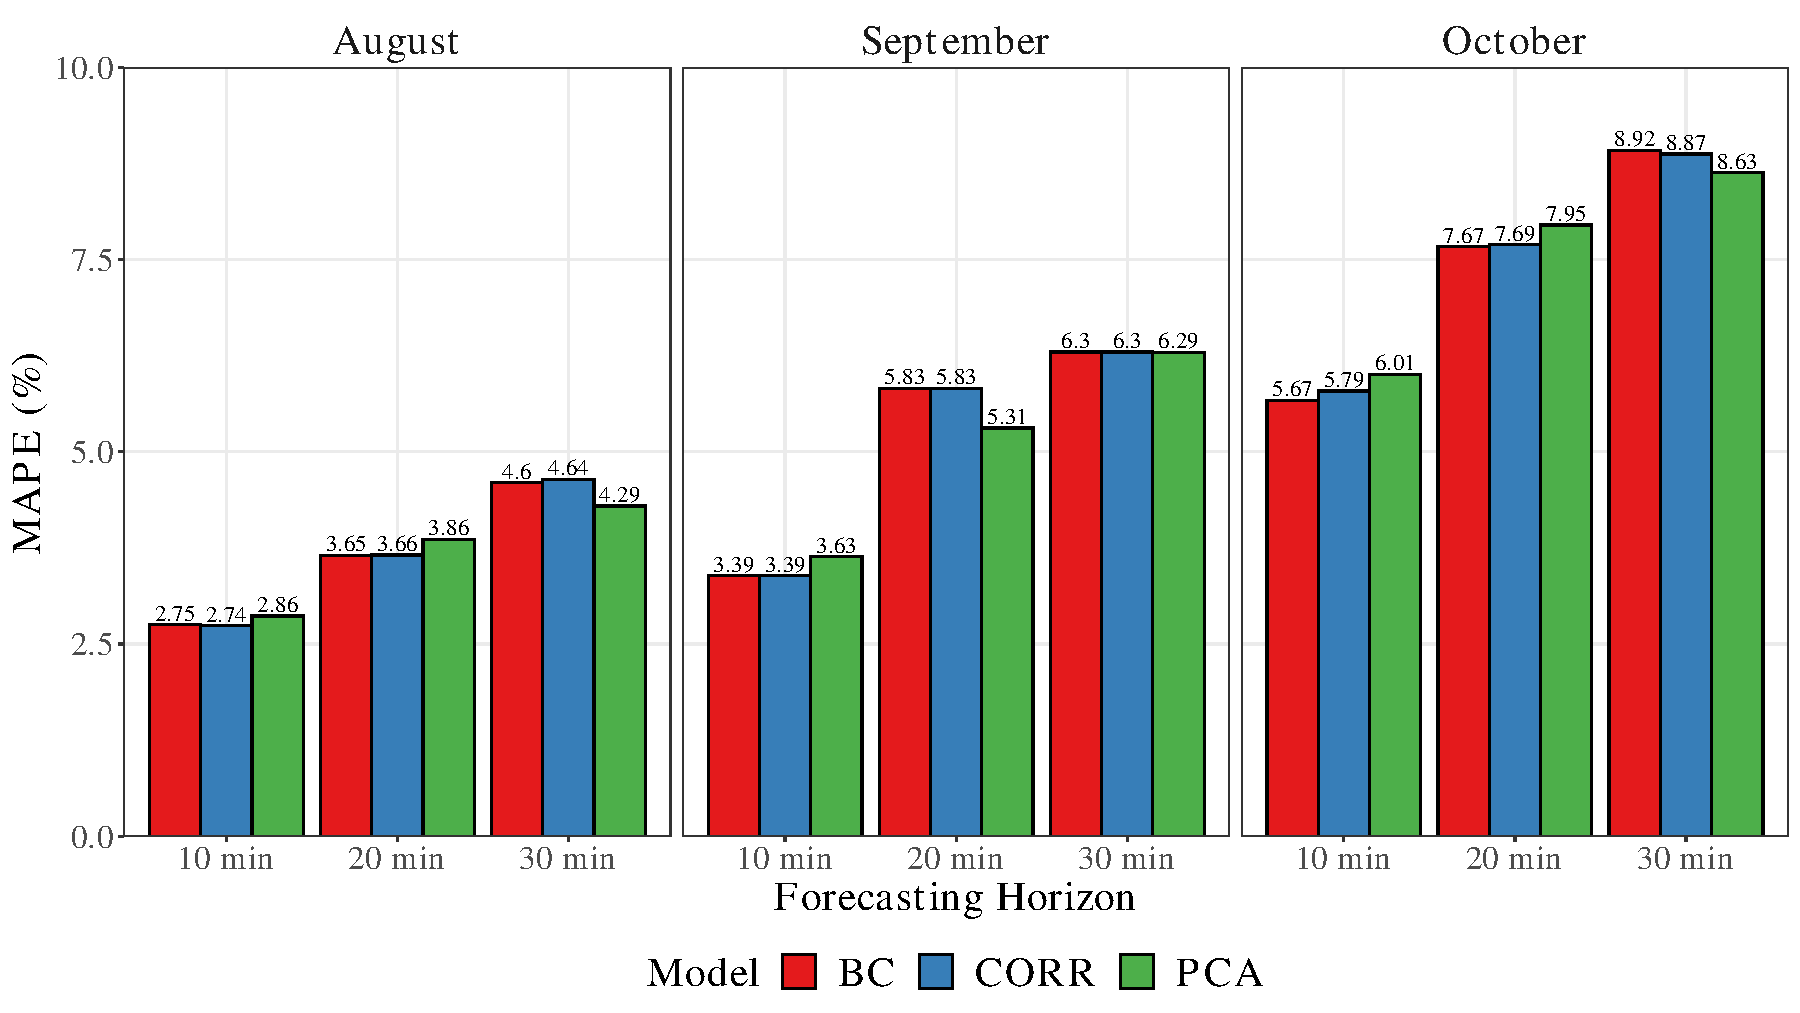
\includegraphics[width=\textwidth]{Media/cs2_mape_barplot.pdf}
    \caption{Evaluated models according to different preprocessing techniques}
    \label{fig:performance}
    \source{\citeonline{dasilva2021Novel}}
\end{figure}

As illustrated in Figure~\ref{fig:performance}, models' performances are similar, with a minimum performance difference between them. Regarding the \ac{MAPE} criterion, \ac{CEEMD}--\ac{BC}--\ac{STACK} outperformed the other models for forecasting 20-minutes-ahead in August and 10 and 20-minutes-ahead in October. \ac{CEEMD}--\ac{CORR}--\ac{STACK} presented a better performance for forecasting 10-minutes-ahead in August, and the same performance 10-minutes-ahead in September. In the remaining scenarios, \ac{CEEMD}--\ac{PCA}--\ac{STACK} performed better.

Even though \ac{CORR} and \ac{PCA} techniques seem to be similar, \ac{CORR}, as a feature selection technique, acts as a filter, selecting and excluding highly correlated or co-linear features that can cause overfitting without changing them \cite{hu2020Multilabel, ma2020Filterbased}. On the other hand, \ac{PCA} is a dimensionality reduction technique that transforms features into a lower dimension, where it is helpful in cases with multicollinearity or where the explanation of predictors is not a priority \cite{marsboom2018Using, salem2019Data}. 

Summarizing, while \ac{CORR} filters the features, \ac{PCA} projects the data into a lower-dimensional space, seeking to find linear combinations of the features. And this can generate a set that, even composed of the combination of existing features, is less efficient than using only those that are not correlated.

Furthermore, the \ac{BC} technique takes advantage of transforming the time series into a normal distribution. With this, the \ac{BC} stabilizes the data variation making the patterns more easily recognizable. Furthermore, stabilizing the variance ensures that the results are not influenced by variability. This allows the meta model (\ac{CUBIST}) to learn more easily when time series patterns become clearer.

\subsection{Comparison with decomposed model \label{subsec:propVSdecomp}}

The second comparison is designed to evaluate the performance of the proposed models by four models based on single decomposition, \ac{CEEMD}--\ac{KNN}, \ac{CEEMD}--\ac{PLS}, \ac{CEEMD}--\ac{RIDGE}, and \ac{CEEMD}--\ac{SVR}. These models performed the decomposition scheme but did not employ the stacking-ensemble learning method. The investigation conducted the comparisons for all forecasting horizons and all datasets.

% % TABLE - CEEMD-STACK versus CEEMD
% {\tiny\tabcolsep=1pt \centering
\begin{longtable}[htb!]{llllllllll}
\caption{Performance measures of the proposed and CEEMD models used to forecast wind power multi-step-ahead \label{tab:PROPversusCEEMD}}\\
\hline
\multirow{2}{*}{\textbf{Dataset}} &
\multirow{2}{*}{\textbf{Forecasting Horizon}} &
\multirow{2}{*}{\textbf{Criteria}} &
\multicolumn{7}{c}{\textbf{Model}} \\ \cline{4-10}
& & & CEEMD--BC--STACK & CEEMD--CORR--STACK & CEEMD--PCA--STACK & CEEMD--KNN & CEEMD--PLS & CEEMD--RIDGE & CEEMD--SVR \\ \hline \endfirsthead

\multicolumn{10}{c}{\tablename\ \thetable\ -- \textit{Continued from previous page}} \\ \hline

\multirow{2}{*}{\textbf{Dataset}} &
\multirow{2}{*}{\textbf{Forecasting Horizon}} &
\multirow{2}{*}{\textbf{Criteria}} &
\multicolumn{7}{c}{\textbf{Model}} \\ \cline{4-10}
& & & CEEMD--BC--STACK & CEEMD--CORR--STACK & CEEMD--PCA--STACK & CEEMD--KNN & CEEMD--PLS & CEEMD--RIDGE & CEEMD--SVR \\ \hline
%
\endhead \hline \multicolumn{10}{r}{\textit{Continued on next page}} \\
\endfoot
\hline
\endlastfoot

{August} &
  {10-minutes-ahead} &
  MAE &
  43.19 &
  \textbf{42.99} &
  44.99 &
  67.63 &
  53.89 &
  50.54 &
  46.89 \\
 &                                   & MAPE & 2.75\%          & \textbf{2.74\%} & 2.86\%          & 4.32\%  & 3.38\%          & 3.11\%   & 2.91\% \\
 &                                   & RMSE & 58.85           & \textbf{58.94}  & 61.53           & 90.16   & 70.95           & 65.09    & 61.21  \\ \cline{2-10}
 & {20-minutes-ahead} & MAE  & \textbf{57.14}  & 57.45           & 60.26           & 76.57   & 68.04           & 205.24   & 82.61  \\
 &                                   & MAPE & \textbf{3.65\%} & 3.66\%          & 3.86\%          & 4.90\%  & 4.27\%          & 10.67\%  & 4.91\% \\
 &                                   & RMSE & \textbf{80.43}  & 80.29           & 84.24           & 102.55  & 90.40           & 320.62   & 110.44 \\ \cline{2-10}
 & {30-minutes-ahead} & MAE  & 72.21           & 72.51           & \textbf{67.03}  & 84.46   & 77.17           & 1,656.42 & 152.20 \\
 &                                   & MAPE & 4.60\%          & 4.64\%          & \textbf{4.29\%} & 5.47\%  & 4.84\%          & -        & 8.26\% \\
 &                                   & RMSE & 96.92           & 98.30           & \textbf{92.11}  & 114.58  & 101.86          & 3,723.23 & 232.88 \\ \hline
{September} &
  {10-minutes-ahead} &
  MAE &
  \textbf{49.56} &
  \textbf{49.56} &
  52.20 &
  80.74 &
  63.38 &
  57.20 &
  52.56 \\
 &                                   & MAPE & \textbf{3.39\%} & \textbf{3.39\%} & 3.63\%          & -       & 4.14\%          & 3.69\%   & 3.46\% \\
 &                                   & RMSE & \textbf{84.16}  & \textbf{84.16}  & 87.69           & 120.75  & 96.47           & 86.50    & 86.05  \\ \cline{2-10}
 &
  {20-minutes-ahead} &
  MAE &
  \textbf{67.46} &
  \textbf{67.46} &
  70.73 &
  88.43 &
  80.06 &
  177.08 &
  82.91 \\
 &                                   & MAPE & 5.83\%          & 5.83\%          & \textbf{5.31\%} & 6.73\%  & 5.31\%          & 12.14\%  & 5.51\% \\
 &                                   & RMSE & \textbf{105.42} & \textbf{105.42} & 109.57          & 128.95  & 116.01          & 264.56   & 119.99 \\ \cline{2-10}
 & {30-minutes-ahead} & MAE  & 80.82           & 80.82           & \textbf{78.52}  & 94.97   & 90.87           & 835.77   & 135.36 \\
 &                                   & MAPE & 6.30\%          & 6.30\%          & 6.29\%          & 7.12\%  & \textbf{5.99\%} & -        & 9.10\% \\
 &                                   & RMSE & 122.75          & 122.75          & \textbf{120.83} & 137.49  & 131.00          & 1,748.88 & 191.45 \\ \hline
{October} &
  {10-minutes-ahead} &
  MAE &
  \textbf{62.25} &
  63.37 &
  66.06 &
  110.81 &
  80.22 &
  70.35 &
  69.90 \\
 &                                   & MAPE & \textbf{5.67\%} & 5.79\%          & 6.01\%          & 9.27\%  & 7.47\%          & 6.42\%   & -      \\
 &                                   & RMSE & \textbf{90.24}  & 92.18           & 94.58           & 150.15  & 110.22          & 98.34    & 101.07 \\ \cline{2-10}
 & {20-minutes-ahead} & MAE  & \textbf{89.18}  & 89.47           & 92.27           & 124.40  & 99.54           & 197.14   & 104.52 \\
 &                                   & MAPE & \textbf{7.67\%} & 7.69\%          & 7.95\%          & 10.23\% & 8.82\%          & -        & 9.27\% \\
 &                                   & RMSE & \textbf{125.55} & 125.77          & 128.60          & 168.90  & 134.63          & 290.97   & 146.31 \\ \cline{2-10}
 &
  {30-minutes-ahead} &
  MAE &
  106.06 &
  104.96 &
  \textbf{101.32} &
  132.09 &
  110.56 &
  692.99 &
  150.62 \\
 &                                   & MAPE & 8.92\%          & 8.87\%          & \textbf{8.63\%} & 10.72\% & 9.72\%          & -        & -      \\
 &                                   & RMSE & 145.52          & 145.24          & \textbf{138.97} & 179.42  & 147.54          & 1,325.83 & 207.63 \\ \hline
\end{longtable}
}


Within the comparisons presented in Table~\ref{tab:PROPversusCEEMD}, the \ac{CEEMD}--\ac{STACK} based models outperformed all other models compared. The worst results were presented by \ac{CEEMD}--\ac{KNN} for August, September, and October in the task of forecasting 10-minutes-ahead, and \ac{CEEMD}--\ac{RIDGE} in the remaining scenarios. The closest results were performed by \ac{CEEMD}--\ac{SVR} for 10-minutes-ahead in all datasets, and \ac{CEEMD}--\ac{PLS} for the other forecasting horizons.

The proposed models outperformed the \ac{CEEMD} models due to the divide-and-conquer approach that the \ac{STACK} method provided. The stacking-ensemble learning method takes advantage of the different learning strategies of each model and uses its best to forecast accurately. Hence, even though \ac{CEEMD}--\ac{RIDGE} presented high errors in the forecasting, its learning characteristics help the ensemble as a whole. The results obtained by the proposed models align with the research carried out by \citeonline{moon2020Combination}, who presented a novel model based on a stacking-ensemble approach to forecast building electric energy consumption. Their model used diverse models to compose the layers of the ensemble learning model, and the proposal outperformed all compared models in all scenarios.

\subsection{Comparison with stacking-ensemble models \label{subsec:propVSstack}}

In this third comparison, the proposed model was compared to the three models that performed the stacking-ensemble learning without decomposing datasets and employed the preprocessing techniques in the layer-1, named \ac{BC}--\ac{STACK}, \ac{CORR}--\ac{STACK}, and \ac{PCA}--\ac{STACK}. As in the previous comparisons, these were conducted for all datasets in all forecasting horizons.

% % TABLE - CEEMD-STACK versus STACK
% {\tiny \tabcolsep=3pt \centering
\begin{longtable}{lllllllll}
\caption{Performance measures of the proposed and STACK models used to forecast wind power multi-step-ahead \label{tab:PROPversusSTACK}}\\
\hline
\multirow{2}{*}{\textbf{Dataset}} & \multirow{2}{*}{\textbf{Forecasting Horizon}} & \multirow{2}{*}{\textbf{Criteria}} & \multicolumn{6}{c}{\textbf{Model}} \\ \cline{4-9}
& & & CEEMD--BC--STACK & CEEMD--CORR--STACK & CEEMD--PCA--STACK & BC--STACK & CORR--STACK & PCA--STACK \\ \hline \endfirsthead

\multicolumn{9}{c}{\tablename\ \thetable\ -- \textit{Continued from previous page}} \\ \hline

\multirow{2}{*}{\textbf{Dataset}} & \multirow{2}{*}{\textbf{Forecasting Horizon}} & \multirow{2}{*}{\textbf{Criteria}} & \multicolumn{6}{c}{\textbf{Model}} \\ \cline{4-9}
& & & CEEMD--BC--STACK & CEEMD--CORR--STACK & CEEMD--PCA--STACK & BC--STACK & CORR--STACK & PCA--STACK \\ \hline
%
\endhead \hline \multicolumn{9}{r}{\textit{Continued on next page}} \\
\endfoot
\hline
\endlastfoot


 
{August}    & {10-minutes-ahead}    & MAE                       & 43.19          & \textbf{42.99} & 44.99 & 113.88 & 113.95 & 113.47 \\
 &                                   & MAPE & 2.75\%           & \textbf{2.74\%}    & 2.86\%            & 7.30\%    & 7.29\%      & 7.29\%     \\
 &                                   & RMSE & 58.85            & \textbf{58.94}     & 61.53             & 153.38    & 153.37      & 153.53     \\ \cline{2-9}
 & {20-minutes-ahead} & MAE  & \textbf{57.14}   & 57.45              & 60.26             & 127.17    & 127.97      & 128.28     \\
 &                                   & MAPE & \textbf{3.65\%}  & 3.66\%             & 3.86\%            & 8.16\%    & 8.20\%      & 8.24\%     \\
 &                                   & RMSE & \textbf{80.43}   & 80.29              & 84.24             & 172.18    & 172.61      & 172.94     \\ \cline{2-9}
 & {30-minutes-ahead} & MAE  & 72.21            & 72.51              & \textbf{67.03}    & 139.86    & 141.44      & 140.94     \\
 &                                   & MAPE & 4.60\%           & 4.64\%             & \textbf{4.29\%}   & 9.02\%    & 9.11\%      & 9.07\%     \\
 &                                   & RMSE & 96.92            & 98.30              & \textbf{92.11}    & 188.32    & 189.70      & 189.20     \\ \hline
{September} & {10-minutes-ahead}    & MAE                       & \textbf{49.56} & \textbf{49.56} & 52.20 & 116.51 & 116.51 & 116.12 \\
 &                                   & MAPE & \textbf{3.39\%}  & \textbf{3.39\%}    & 3.63\%            & 7.28\%    & 7.28\%      & 7.28\%     \\
 &                                   & RMSE & \textbf{84.16}   & \textbf{84.16}     & 87.69             & 166.86    & 166.85      & 165.87     \\ \cline{2-9}
                           & {20-minutes-ahead}    & MAE                       & \textbf{67.46} & \textbf{67.46} & 70.73 & 127.61 & 127.94 & 127.30 \\
 &                                   & MAPE & 5.83\%           & 5.83\%             & \textbf{5.31\%}   & 7.91\%    & 7.91\%      & 7.91\%     \\
 &                                   & RMSE & \textbf{105.42}  & \textbf{105.42}    & 109.57            & 182.09    & 182.41      & 181.60     \\ \cline{2-9}
 & {30-minutes-ahead} & MAE  & 80.82            & 80.82              & \textbf{78.52}    & 141.13    & 136.13      & 135.68     \\
 &                                   & MAPE & 6.30\%           & 6.30\%             & \textbf{6.29\%}   & 8.82\%    & 8.36\%      & 8.32\%     \\
 &                                   & RMSE & 122.75           & 122.75             & \textbf{120.83}   & 196.94    & 192.66      & 192.42     \\ \hline
{October}   & {10-minutes-ahead}    & MAE                       & \textbf{62.25} & 63.37          & 66.06 & 159.53 & 160.47 & 157.49 \\
 &                                   & MAPE & \textbf{5.67\%}  & 5.79\%             & 6.01\%            & 12.85\%   & 12.79\%     & 12.66\%    \\
 &                                   & RMSE & \textbf{90.24}   & 92.18              & 94.58             & 215.91    & 216.09      & 212.58     \\ \cline{2-9}
 & {20-minutes-ahead} & MAE  & \textbf{89.18}   & 89.47              & 92.27             & 176.98    & 178.85      & 177.50     \\
 &                                   & MAPE & \textbf{7.67\%}  & 7.69\%             & 7.95\%            & 13.97\%   & 14.11\%     & 14.06\%    \\
 &                                   & RMSE & \textbf{125.55}  & 125.77             & 128.60            & 238.15    & 240.80      & 238.74     \\ \cline{2-9}
 & {30-minutes-ahead} & MAE  & 106.06           & 104.96             & \textbf{101.32}   & 194.55    & 193.00      & 191.40     \\
 &                                   & MAPE & 8.92\%           & 8.87\%             & \textbf{8.63\%}   & 15.30\%   & 15.15\%     & 15.10\%    \\
 &                                   & RMSE & 145.52           & 145.24             & \textbf{138.97}   & 258.72    & 257.82      & 254.91     \\ \hline
\end{longtable}
}

Table~\ref{tab:PROPversusSTACK} presents the performance measures of the proposed forecasting framework and the \ac{STACK} models. The proposed models outperformed the compared models in the performance criteria. The \ac{STACK} models presented quite similar performance among them, with a minimum difference in the performance criteria in all datasets for all forecasting horizons.

Regardless of the advantages of the \ac{STACK} method, the proposed models still present better performance compared to \ac{STACK} models without the \ac{CEEMD} preprocessing. This is due to the \ac{CEEMD} method that deals with the non-linearity and non-stationarity of the wind power generation data and completely neutralizes the residual noise-producing an improved forecasting method. In contrast, the \ac{STACK} method is not able by itself to deal with the fluctuations and unstable demand of wind energy, which makes it difficult to forecast accurately without preprocessing the data, using a decomposition method, for example. The results obtained by the proposed model corroborate with the findings from \citeonline{niu2020Shortterm}, who successfully applied \ac{CEEMD} into a photovoltaic power generation time series, once the \ac{CEEMD} method can effectively decompose an unstable time series into stable sub-sequences to weaken the fluctuation of the original signal.

\subsection{Comparison with non-decomposed models \label{subsec:propVSmodels}}

Finally, the investigation compared the proposed with non-decomposed models, named \ac{KNN}, \ac{PLS}, \ac{RIDGE}, and \ac{SVR}. The performance measures of the models are presented in Table~\ref{tab:PROPversusMODELS}.

% % TABLE - CEEMD-STACK versus MODELS
% {\tiny \tabcolsep=3pt \centering
\begin{longtable}[htb!]{llllllllll}
\caption{Performance measures of the proposed and machine learning models used to forecast wind power multi-step-ahead \label{tab:PROPversusMODELS}} \\

\hline
\multirow{2}{*}{\textbf{Dataset}} & \multirow{2}{*}{\textbf{Forecasting Horizon}} & \multirow{2}{*}{\textbf{Criteria}} & \multicolumn{7}{c}{\textbf{Model}} \\ \cline{4-10}
& & & CEEMD--CORR--STACK & CEEMD--PCA--STACK & CEEMD--BC--STACK & KNN & PLS & RIDGE & SVR \\ \hline \endfirsthead

\multicolumn{10}{c}{\tablename\ \thetable\ -- \textit{Continued from previous page}} \\ \hline

\multirow{2}{*}{\textbf{Dataset}} & \multirow{2}{*}{\textbf{Forecasting Horizon}} & \multirow{2}{*}{\textbf{Criteria}} & \multicolumn{7}{c}{\textbf{Model}} \\ \cline{4-10}
& & & CEEMD--CORR--STACK & CEEMD--PCA--STACK & CEEMD--BC--STACK & KNN & PLS & RIDGE & SVR \\ \hline

\endhead \hline \multicolumn{10}{r}{\textit{Continued on next page}} \\
\endfoot
\hline
\endlastfoot

{August}    & {10-minutes-ahead}    & MAE                       & 43.19              & \textbf{42.99}    & 44.99            & 121.87  & 109.15  & 109.19  & 108.68  \\
                           &                                      & MAPE                      & 2.75\%             & \textbf{2.74\%}   & 2.86\%           & 7.81\%  & 7.02\%  & 7.02\%  & 6.95\%  \\
                           &                                      & RMSE                      & 58.85              & \textbf{58.94}    & 61.53            & 159.55  & 147.91  & 147.90  & 147.91  \\ \cline{2-10}
                           & {20-minutes-ahead}    & MAE                       & \textbf{57.14}     & 57.45             & 60.26            & 132.07  & 123.24  & 123.06  & 122.81  \\
                           &                                      & MAPE                      & \textbf{3.65\%}    & 3.66\%            & 3.86\%           & 8.48\%  & 7.97\%  & 7.95\%  & 7.86\%  \\
                           &                                      & RMSE                      & \textbf{80.43}     & 80.29             & 84.24            & 174.21  & 168.23  & 168.11  & 168.71  \\ \cline{2-10}
                           & {30-minutes-ahead}    & MAE                       & 72.21              & 72.51             & \textbf{67.03}   & 142.29  & 135.20  & 134.73  & 135.46  \\
                           &                                      & MAPE                      & 4.60\%             & 4.64\%            & \textbf{4.29\%}  & 9.18\%  & 8.75\%  & 8.72\%  & 8.65\%  \\
                           &                                      & RMSE                      & 96.92              & 98.30             & \textbf{92.11}   & 188.35  & 181.36  & 181.14  & 182.08  \\ \hline
{September} & {10-minutes-ahead}    & MAE                       & \textbf{49.56}     & \textbf{49.56}    & 52.20            & 125.71  & 114.92  & 113.71  & 113.02  \\
                           &                                      & MAPE                      & \textbf{3.39\%}    & \textbf{3.39\%}   & 3.63\%           & 7.79\%  & 7.44\%  & 7.37\%  & 7.32\%  \\
                           &                                      & RMSE                      & \textbf{84.16}     & \textbf{84.16}    & 87.69            & 174.80  & 163.62  & 162.82  & 164.33  \\ \cline{2-10}
                           & {20-minutes-ahead}    & MAE                       & \textbf{67.46}     & \textbf{67.46}    & 70.73            & 133.43  & 125.47  & 123.33  & 122.82  \\
                           &                                      & MAPE                      & 5.83\%             & 5.83\%            & \textbf{5.31\%}  & 8.26\%  & 7.94\%  & 7.78\%  & 7.77\%  \\
                           &                                      & RMSE                      & \textbf{105.42}    & \textbf{105.42}   & 109.57           & 186.85  & 176.05  & 174.42  & 177.99  \\ \cline{2-10}
                           & {30-minutes-ahead}    & MAE                       & 80.82              & 80.82             & \textbf{78.52}   & 137.56  & 133.86  & 130.69  & 128.87  \\
                           &                                      & MAPE                      & 6.30\%             & 6.30\%            & \textbf{6.29\%}  & 8.52\%  & 8.46\%  & 8.24\%  & 8.15\%  \\
                           &                                      & RMSE                      & 122.75             & 122.75            & \textbf{120.83}  & 192.22  & 182.71  & 181.04  & 183.85  \\ \hline
{October}   & {10-minutes-ahead}    & MAE                       & \textbf{62.25}     & 63.37             & 66.06            & 163.35  & 149.43  & 149.39  & 148.79  \\
                           &                                      & MAPE                      & \textbf{5.67\%}    & 5.79\%            & 6.01\%           & 13.13\% & 12.36\% & 12.40\% & 12.54\% \\
                           &                                      & RMSE                      & \textbf{90.24}     & 92.18             & 94.58            & 218.68  & 200.72  & 200.70  & 202.84  \\ \cline{2-10}
                           & {20-minutes-ahead}    & MAE                       & \textbf{89.18}     & 89.47             & 92.27            & 176.68  & 161.27  & 161.26  & 160.11  \\
                           &                                      & MAPE                      & \textbf{7.67\%}    & 7.69\%            & 7.95\%           & 14.11\% & 13.26\% & 13.30\% & 13.51\% \\
                           &                                      & RMSE                      & \textbf{125.55}    & 125.77            & 128.60           & 236.81  & 218.07  & 217.81  & 221.76  \\ \cline{2-10}
                           & {30-minutes-ahead}    & MAE                       & 106.06             & 104.96            & \textbf{101.32}  & 191.75  & 172.48  & 171.96  & 172.69  \\
                           &                                      & MAPE                      & 8.92\%             & 8.87\%            & \textbf{8.63\%}  & 15.22\% & 13.94\% & 13.94\% & 14.15\% \\
                           &                                      & RMSE                      & 145.52             & 145.24            & \textbf{138.97}  & 254.62  & 229.21  & 228.53  & 233.66  \\ \hline
\end{longtable}
}

This comparison also presented behavior similar to previous comparisons. Indeed the proposed model outperformed the stand-alone machine learning models for all datasets in all forecasting horizons in all metrics. In this comparison, the \ac{KNN} model presented the worst performance for all datasets in all forecasting horizons. 

As expected, the single models could not deal with the complexity of wind power generation data. Compared to the proposed models, the single models seem inefficient. On the other hand, when preprocessed and combined as an ensemble learning method, each approach can learn different characteristics and extract its best to build an accurate and efficient forecasting model. Regarding this, \citeonline{moon2020Combination} and \citeonline{ribeiro2020Shortterm} showed that \ac{STACK} models indeed present better results than single models, as previously highlighted that is due to the divide-and-conquer approach, where different methods could learn different patterns and behaviors to generate an accurate forecasting performance. Nevertheless, \citeonline{zhang2020Novel} and \citeonline{ali2020Complete} presented comparisons of the \ac{CEEMD} model forecasting performance in the face of the single model performance. The \ac{CEEMD} approach dealt with the non-stationarity and non-linearity behaviors faced by the financial and weather time series by weakening the fluctuation of the signals once the approach can resolve and isolate the significant fluctuating signals into respective smaller frequency components.

\subsection{Hypothesis tests \label{subsec:stastistical}}

The \ac{DM} tests were conducted to compare the most accurate model, which presented better performance, to the other models, for each dataset in all forecasting horizons. Table~\ref{tab:DMtest} presents the DM-values. The \ac{DM} test results prove that the proposed models performed better than all the models in all given scenarios once the DM-values presented negative values.

% % TABLE - DM TEST
% {\tiny\tabcolsep=1pt \centering
\begin{longtable}{llll|lll|lll}
\caption{Statistics of DM test for statistical comparison of proposed approach versus other models \label{tab:DMtest}} \\

\hline
\multirow{3}{*}{\textbf{Model}} & \multicolumn{3}{c|}{\textbf{August}}        & \multicolumn{3}{c|}{\textbf{September}} & \multicolumn{3}{c}{\textbf{October}} \\ \cline{2-10}
&
10-min-ahead &
20-min-ahead &
30-min-ahead &
10-min-ahead &
20-min-ahead &
30-min-ahead &
10-min-ahead &
20-min-ahead &
30-min-ahead \\ \cline{2-10}
& (B) & (A) & (C) & (B) & (B) & (C) & (A) & (A) & (C) \\ \hline \endfirsthead

\multicolumn{10}{c}{\tablename\ \thetable\ -- \textit{Continued from previous page}} \\ \hline

\hline
\multirow{3}{*}{\textbf{Model}} & \multicolumn{3}{c|}{\textbf{August}}        & \multicolumn{3}{c|}{\textbf{September}} & \multicolumn{3}{c}{\textbf{October}} \\ \cline{2-10}
&
10-min-ahead &
20-min-ahead &
30-min-ahead &
10-min-ahead &
20-min-ahead &
30-min-ahead &
10-min-ahead &
20-min-ahead &
30-min-ahead \\ \cline{2-10}
& (B) & (A) & (C) & (B) & (B) & (C) & (A) & (A) & (C) \\ \hline 

\endhead \hline \multicolumn{10}{r}{\textit{Continued on next page}} \\
\endfoot
\endlastfoot

(A) CEEMD--BC--STACK   & -1.2783   & -         & -5.9698*  & -         & -         & -2.3487** & -         & -         & -5.7326*  \\
(B) CEEMD--CORR--STACK & -         & -0.9416   & -6.7649*  & -         & -         & -2.3487** & -5.7868*  & -1.8874   & -3.0929*  \\
(C) CEEMD--PCA--STACK  & -5.3166*  & -4.7033*  & -         & -4.7040*  & -3.3635*  & -         & -6.3865*  & -3.2087*  & -         \\  \hline
(D) CEEMD--KNN         & -17.3931* & -14.7071* & -11.5924* & -14.8768* & -11.3851* & -8.3644*  & -18.1568* & -15.6918* & -12.3660* \\
(E) CEEMD--PLS         & -10.8987* & -7.4707*  & -5.9180*  & -11.1695* & -7.1736*  & -6.7370*  & -12.1801* & -4.1905*  & -3.1324*  \\
(F) CEEMD--RIDGE       & -9.4215*  & -28.5236* & -24.0609* & -7.7562*  & -29.7477* & -23.3920* & -6.9984*  & -20.9568* & -23.6192* \\
(G) CEEMD--SVR         & -5.3697*  & -11.5289* & -13.5758* & -3.0116*  & -8.6876*  & -17.9531* & -6.7004*  & -4.7606*  & -9.3912*  \\ \hline
(H) BC--STACK          & -23.9344* & -17.4176* & -13.4572* & -18.9641* & -14.2140* & -11.2585* & -22.1231* & -17.7841* & -15.6152* \\
(I) CORR--STACK        & -23.9576* & -17.5908* & -13.7338* & -18.8531* & -14.1175* & -10.7107* & -22.3690* & -18.0238* & -15.2418* \\
(J) PCA--STACK         & -23.6773* & -17.4651* & -13.5909* & -18.9014* & -14.2366* & -10.6806* & -21.9771* & -17.9894* & -15.2968* \\ \hline
(K) KNN                & -25.9367* & -18.6722* & -14.2327* & -20.1948* & -14.8886* & -11.1571* & -22.7918* & -18.1020* & -15.4478* \\
(L) PLS                & -22.9573* & -17.6782* & -14.3770* & -19.2370* & -15.6723* & -11.9274* & -22.1817* & -17.2128* & -14.3436* \\
(M) RIDGE              & -23.0216* & -17.5853* & -14.2087* & -18.9618* & -14.9467* & -11.2234* & -22.1934* & -17.1000* & -14.0634* \\
(N) SVR                & -22.7365* & -17.5476* & -14.7579* & -18.6710* & -14.3288* & -10.1985* & -21.5547* & -16.2012* & -13.8350* \\ \hline
\multicolumn{10}{l}{\textbf{Note:} *1\% significance level; **5\% significance level.}                                                     
\end{longtable}
}

Regarding the DM-values and $p$-values analyzed, they show that (i) for August forecasting 10-minutes-ahead, the \ac{CEEMD}--\ac{CORR}--\ac{STACK} has similar behavior that \ac{CEEMD}--\ac{BC}--\ac{STACK}. For 20-minutes-ahead forecasting, the \ac{CEEMD}--\ac{BC}--\ac{STACK} is statistically equal to \ac{CEEMD}--\ac{CORR}--\ac{STACK}. Forecasting 30-minutes-ahead the \ac{CEEMD}--\ac{PCA}--\ac{STACK} has no statistical equality with any model; (ii) for September, model \ac{CEEMD}--\ac{CORR}--\ac{STACK} presented no statistical equality with any model when forecasting 10 and 20-minutes-ahead, same for \ac{CEEMD}--\ac{PCA}--\ac{STACK} for forecasting 30-minutes-ahead; and (iii) for October forecasting 10-minutes-ahead, the \ac{CEEMD}--\ac{BC}--\ac{STACK} equals no model, 20-minutes-ahead, the \ac{CEEMD}--\ac{BC}--\ac{STACK} equals to \ac{CEEMD}--\ac{CORR}--\ac{STACK}, and 30-minutes-ahead, \ac{CEEMD}--\ac{PCA}--\ac{STACK} equals to no model as well. Despite these results, it is important to emphasize that even though the errors of some models are statistically the same, the results obtained by using them are not.

\subsection{Graphical analysis \label{subsec:graphical}}

The figures were developed to analyze the errors' standard deviation of the proposed and compared model. The models are labeled in the Figure~\ref{fig:radarplotcs2} as: (A) \ac{CEEMD}--\ac{BC}--\ac{STACK}, (B) \ac{CEEMD}--\ac{CORR}--\ac{STACK}, (C) \ac{CEEMD}--\ac{PCA}--\ac{STACK}, (D) \ac{CEEMD}--\ac{KNN}, (E) \ac{CEEMD}--\ac{PLS}, (F) \ac{CEEMD}--\ac{RIDGE}, (G) \ac{CEEMD}--\ac{SVR}, (H) \ac{BC}--\ac{STACK}, (I) \ac{CORR}--\ac{STACK}, (J) \ac{PCA}--\ac{STACK}, (K) \ac{KNN}, (L) \ac{PLS}, (M) \ac{RIDGE}, and (N) \ac{SVR}. It is important to highlight that (F) \ac{CEEMD}--\ac{RIDGE} was suppressed from the radar plot due to its high error standard deviation, which deformed the plot and made it difficult to read the other analysis.

% FIGURE - Radar plots
\begin{figure}[htb!]
    \centering
    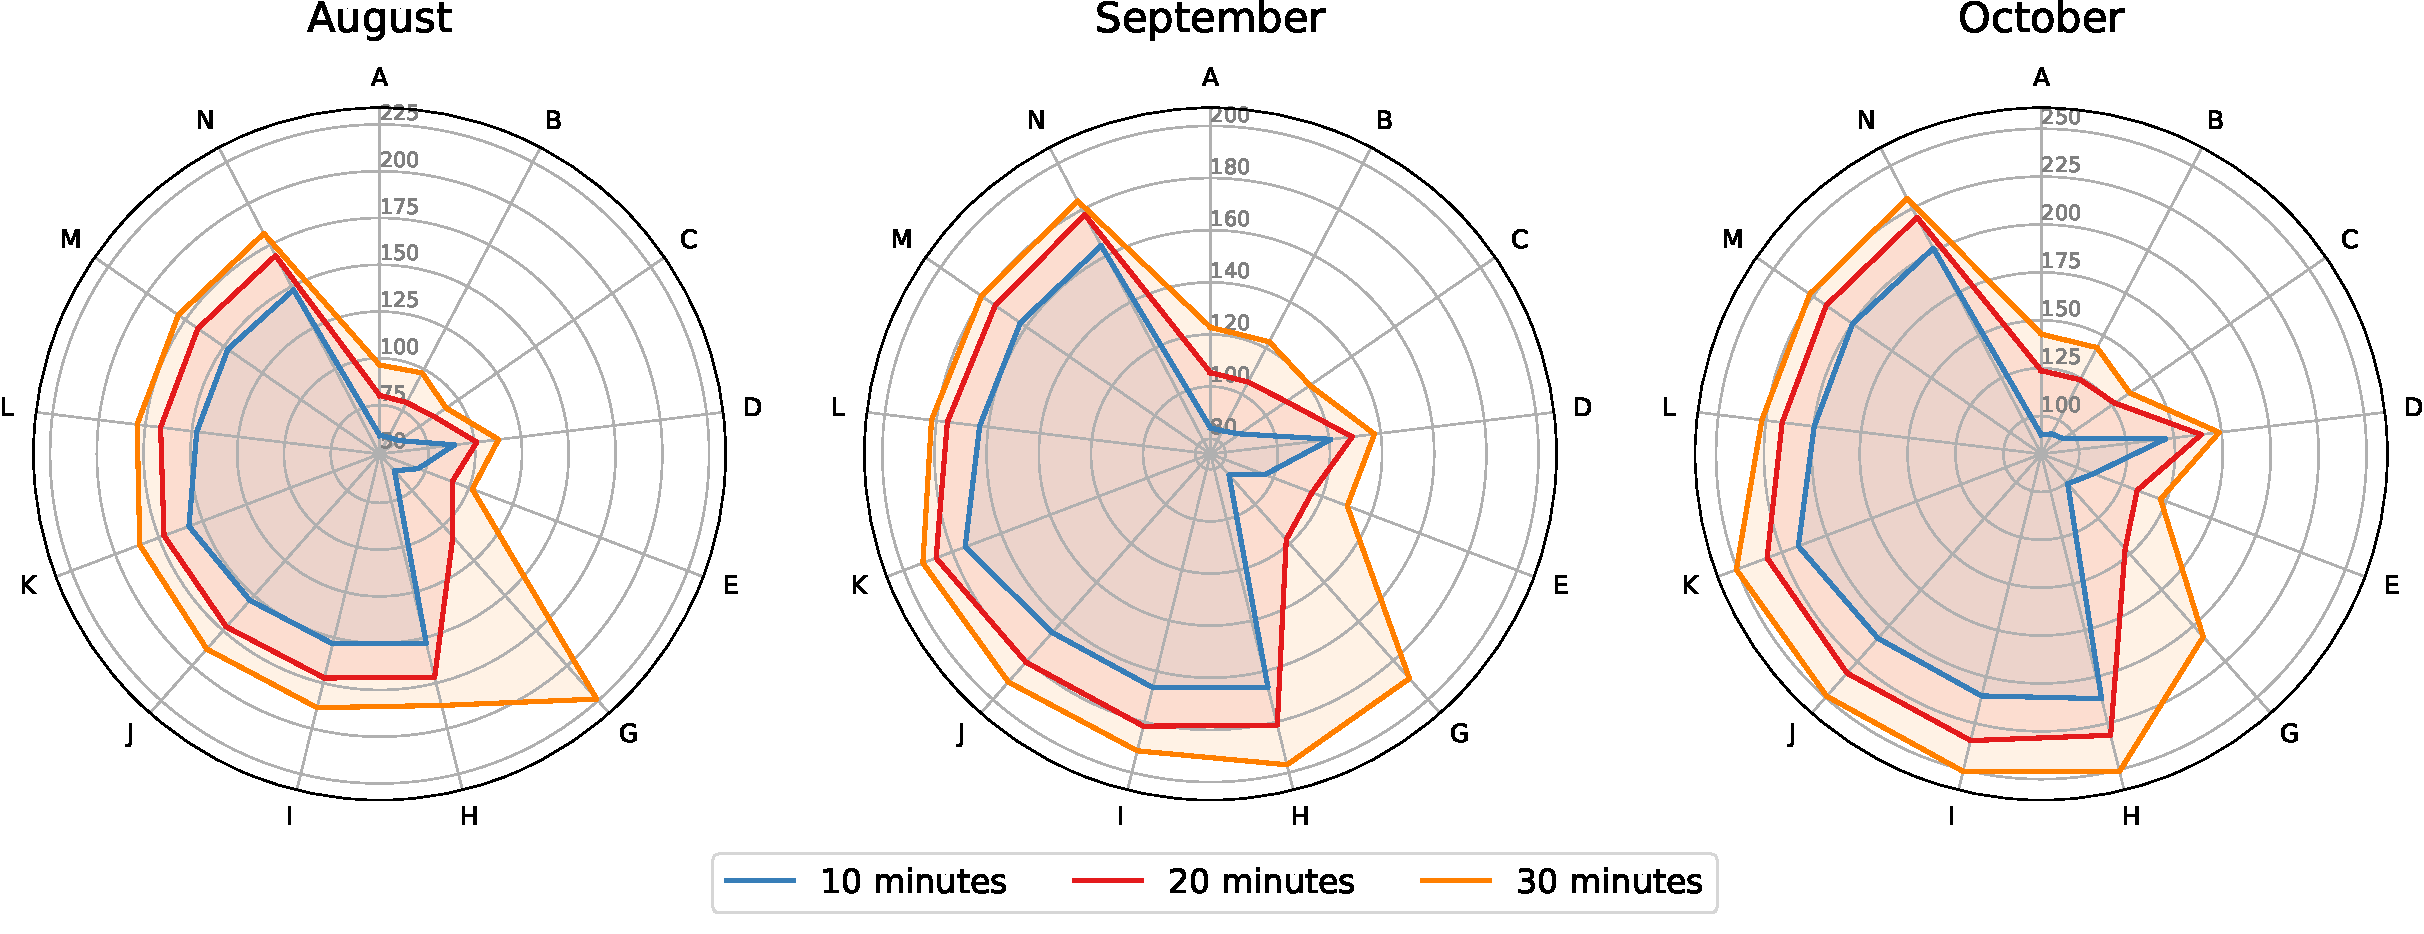
\includegraphics[width=\linewidth]{Media/cs2_radarplot.pdf}
    \caption{Errors' standard deviation for each model}
    \label{fig:radarplotcs2}
    \source{\citeonline{dasilva2021Novel}}
\end{figure}

According to the radar plots of errors' standard deviation, the three proposed models presented higher stability and lower errors for all datasets in all forecasting horizons. This means the proposed forecasting framework learned better than any developed forecasting model in this study.

Furthermore, based on the presented performance measures and statistical results, the \ac{CEEMD}--\ac{BC}--\ac{STACK} is the most accurate model for the August 20-minutes-ahead, and October 10 and 20-minutes-ahead. \ac{CEEMD}--\ac{CORR}--\ac{STACK} is the most accurate model for the August 10-minutes-ahead, and September 10 and 20-minutes-ahead. And \ac{CEEMD}--\ac{PCA}--\ac{STACK} is the most accurate model for August, September, and October 30-minutes-ahead. Figures~\ref{fig:pred-Aug},~\ref{fig:pred-Sep}, and~\ref{fig:pred-Oct} present the out-of-sample (last seven days of the month) in the blue line, versus the predictions in red line for 10, 20, and 30-minutes-ahead, for August, September, and October, respectively.

Regarding the predicted versus observed values of the wind power generation, the proposed framework learned the data behavior, allowing forecasting accurate values compatible with the observed time series. However, the proposed forecasting framework presented difficulties in following the extremes of the data variability even though the results indicate that the hybrid decomposition-ensemble learning model can predict accurate values for wind power generation for different datasets in different forecasting horizons.


% FIGURE - Predictions August
\begin{figure}[htb!]
    \centering
    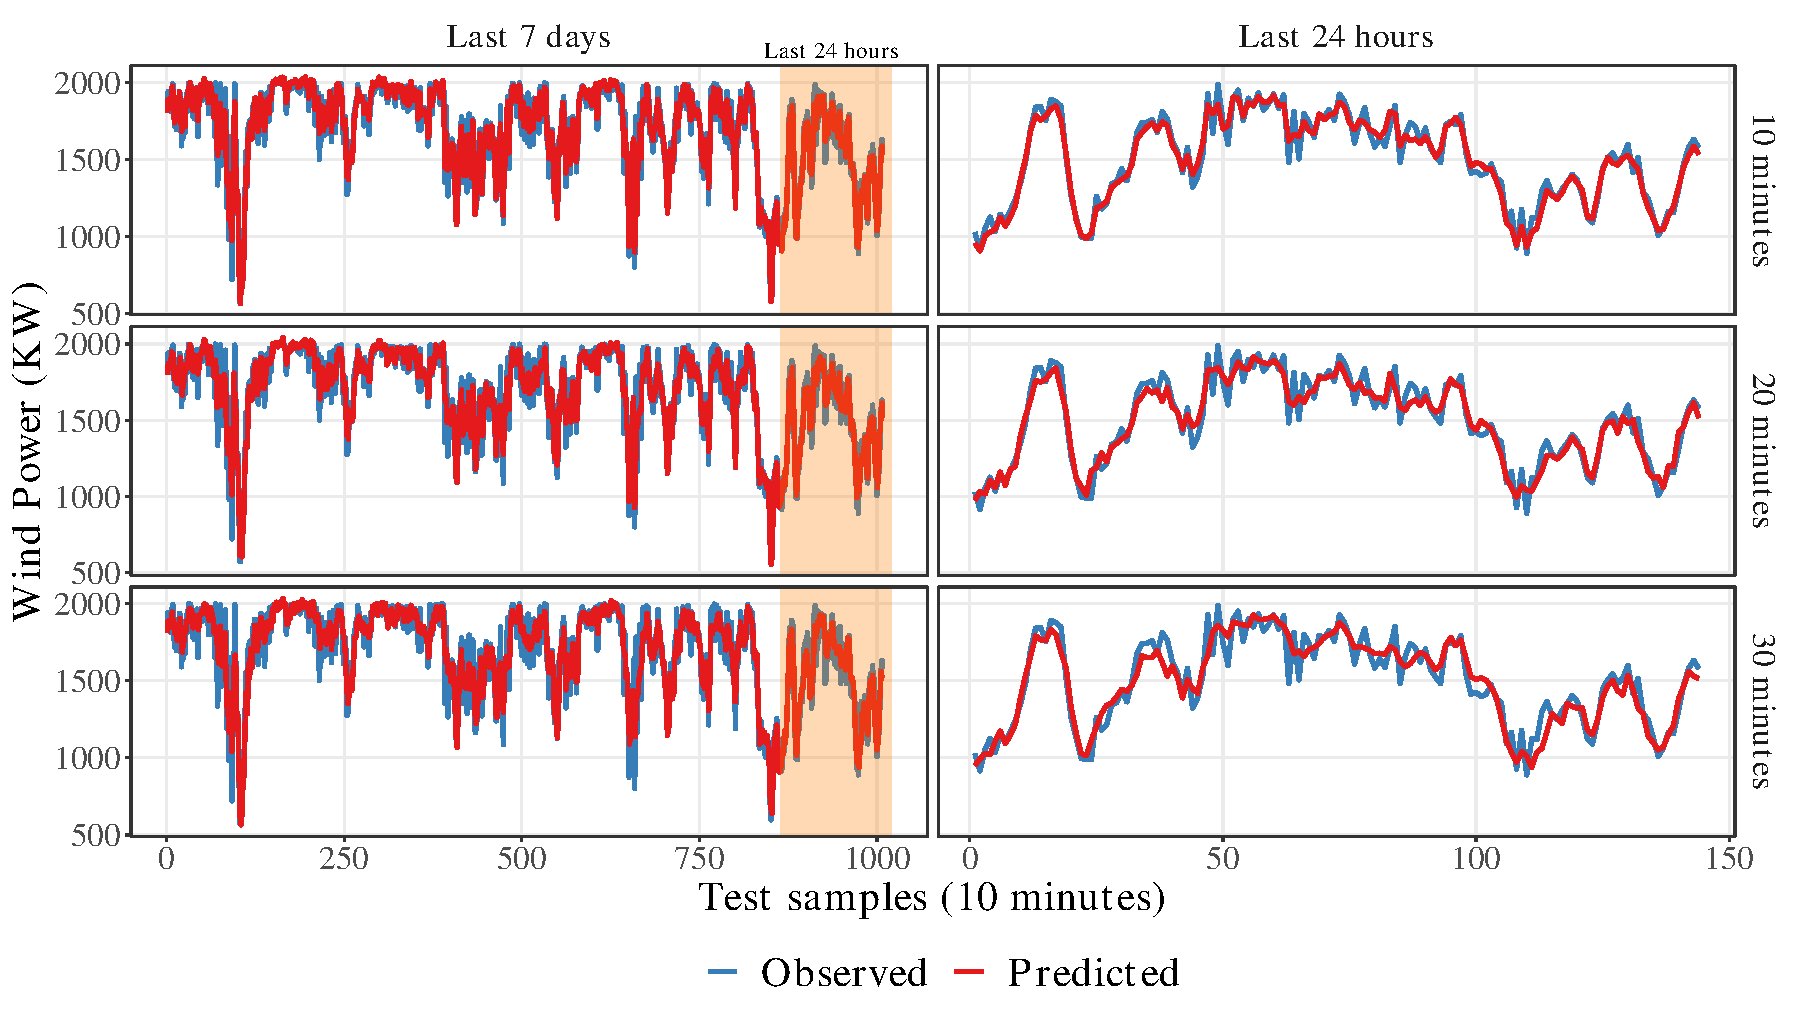
\includegraphics[width=\linewidth]{Media/cs2_PO_2017-08.pdf}
    \caption{Observed versus predictions values for August's test set}
    \label{fig:pred-Aug}
    \source{\citeonline{dasilva2021Novel}}
\end{figure}

% FIGURE - Predictions September
\begin{figure}[htb!]
    \centering
    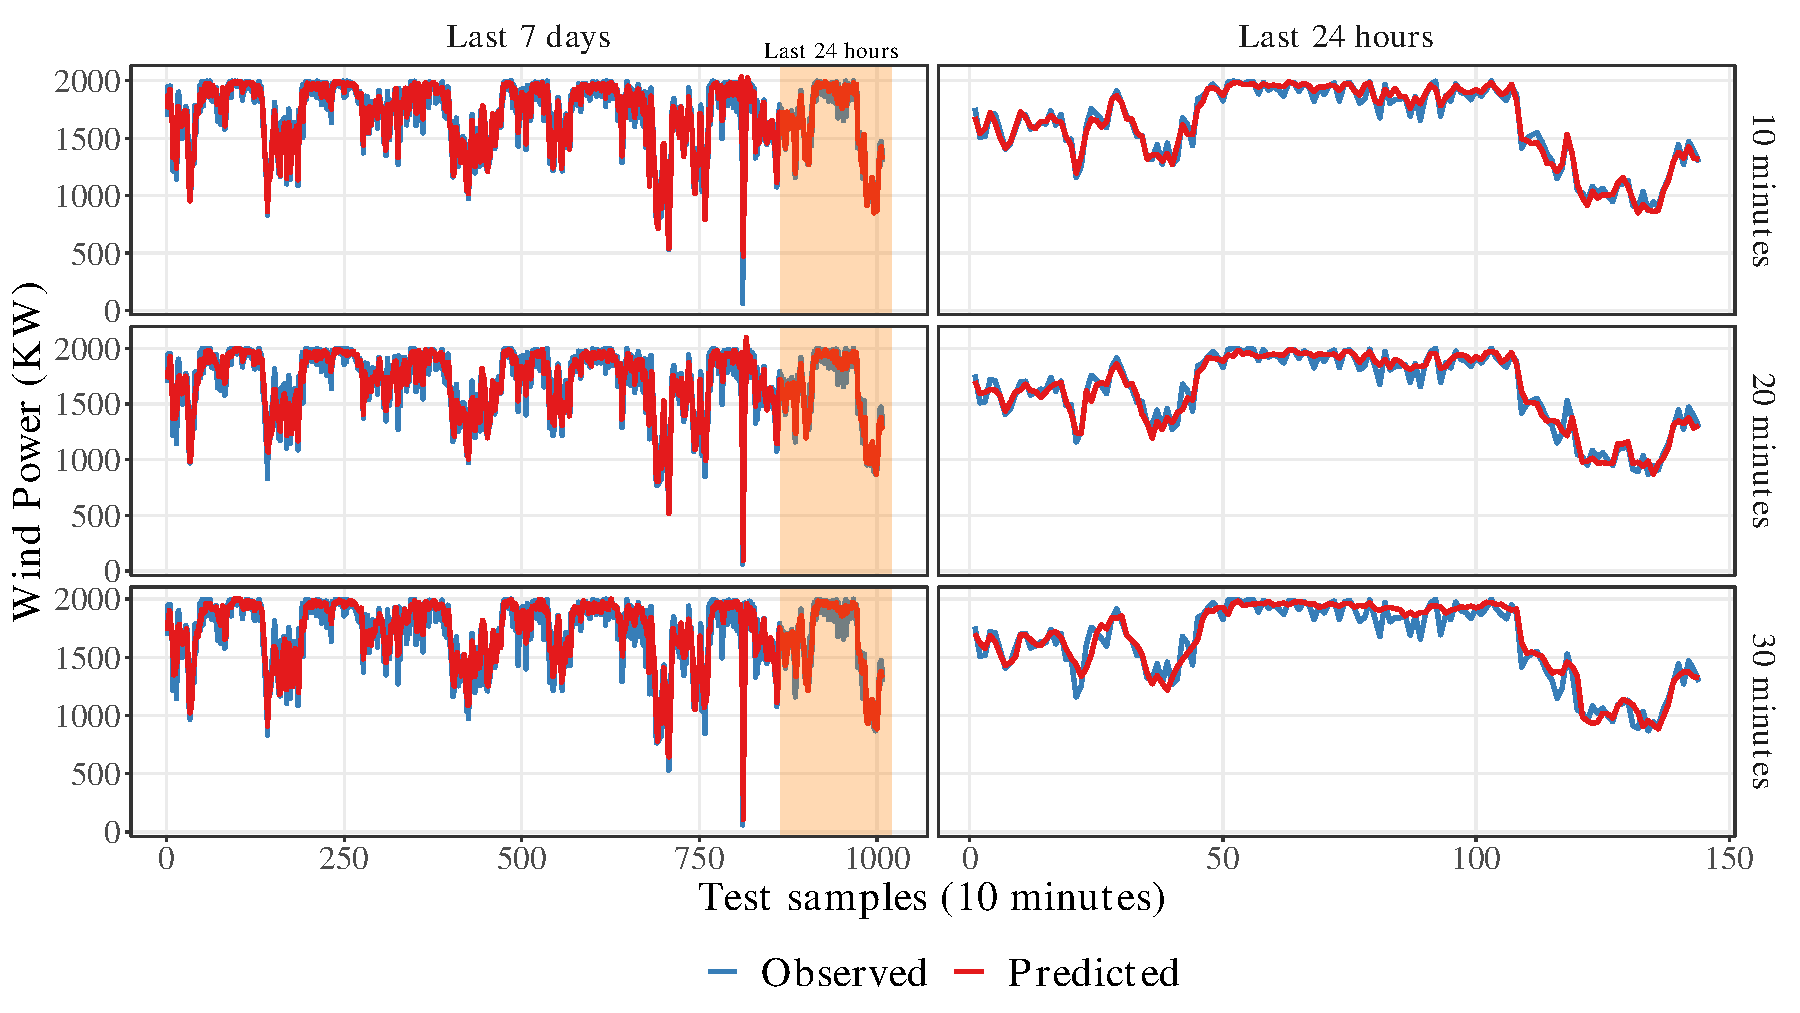
\includegraphics[width=\linewidth]{Media/cs2_PO_2017-09.pdf}
    \caption{Observed versus predictions values for September's test set}
    \label{fig:pred-Sep}
    \source{\citeonline{dasilva2021Novel}}
\end{figure}

% FIGURE - Predictions October
\begin{figure}[htb!]
    \centering
    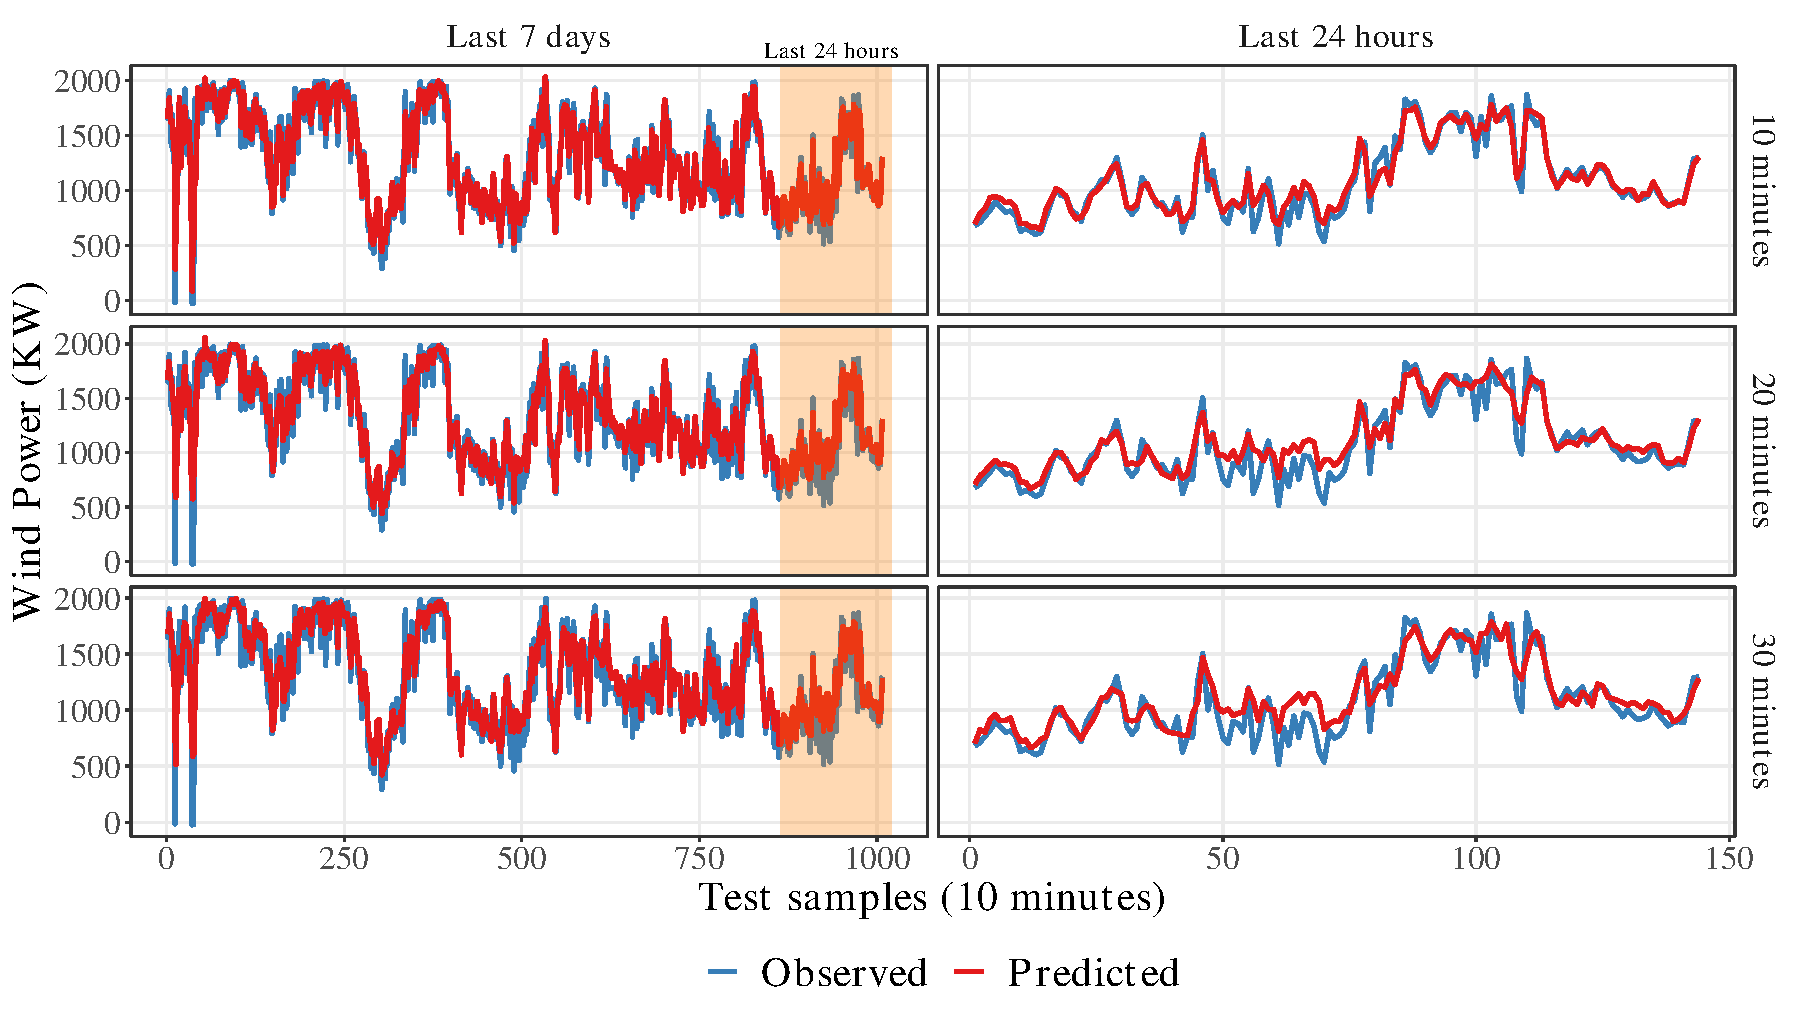
\includegraphics[width=\linewidth]{Media/cs2_PO_2017-10.pdf}
    \caption{Observed versus predictions values for October's test set}
    \label{fig:pred-Oct}
    \source{\citeonline{dasilva2021Novel}}
\end{figure}

\subsection{Conclusions of the Application 2}

This study proposed a hybrid decomposition-ensemble learning model of multi-step-ahead forecasting for very short-term wing energy forecasting. The proposed forecasting framework employed \ac{CEEMD} technique to decompose the data. Each component was trained and fitted with four well-known machine learning models. The predictions of the components were grouped by trained models and summed to generate four models. In the stacking-ensemble layer-1, the data is preprocessed by \ac{BC}, \ac{CORR}, and \ac{PCA} and trained using \ac{CUBIST} as meta-learner. The proposed framework generated three final predictions, and the more accurate is chosen, according to \ac{MAE}, \ac{MAPE}, and \ac{RMSE} performance metrics, as well as \ac{DM} test. Then, the chosen one is compared to decomposed, stacking-ensemble, and single models.

According to the results, it can be concluded that regarding \textbf{RQ 1.2} - \textit{Can signal decomposition approaches enhance the performance of forecasting wind energy generation time series?} and \textbf{RQ 3.1} - \textit{What is the improvement achieved by employing the \ac{STACK} approach coupled with signal decomposition approaches over non-decomposed models when forecasting wind energy generation time series?}, signal decomposition models outperform decomposed, stacking-ensemble, and non-decomposed models. Due to the divide-and-conquer scheme, the stacking-ensemble learning enhanced the accuracy of the weak \ac{CEEMD} models by combining and using them to forecast with a strong model, giving more robustness and stability to the model, even though some weak models presented high errors and low accuracy. Regarding \textbf{RQ 4} - \textit{Can preprocessing methods applied to the time series improve the forecasting performance of the decomposition-ensemble learning strategy?}, the preprocessing techniques improved the performance of the forecasts. They transform the time series making the learning process of the models easier due to their characteristics of filtering highly correlated features or reducing the number of dimensions and then removing multicollinearity from the features. It can be highlighted that the \ac{BC} method outperformed other models in five out of nine scenarios, according to Table \ref{tab:DMtest}. By answering theses \ac{RQ}s, the specific objectives \textbf{\ref{obj_a}}, \textbf{\ref{obj_b}}, and \textbf{\ref{obj_d}} were achieved.